\documentclass[Main]{subfiles}
\begin{document}

\chapter{Software}
Dette kapitel beskriver softwarens opbygning efter 4+1 modellen\cite[p. 872-875]{Larman} og bygger på Kravspecifikationen\cite{KravSpec}. 
Opbygning med 4+1 modellen gør det nemmere at forstå hvordan systemet er sat sammen, da der visse blokke (views) af systemet, der derefter åbnes op.
Derudover kan blokke der ikke er brug for undværes.

Følgende views er valgt:
Logical view, deployment view, process view og implementation view.
Foruden disse er der også valgt et afsnit med nogle designbeslutninger der blev truffet undervejs i forløbet.
\begin{itemize}
\item Logical view beskriver hvordan systemet er opbygget, med diagrammer og funktionsbeskrivelser.
\item Deployment view beskriver det samlede system.
\item Process view beskriver kommunikationen mellem de overordnede dele i systemet.
\item Implementation view beskriver hvordan systemet er bygget og hvad der skal til for, at bygge det på en anden computer.
\end{itemize}

Alle sekvens-diagrammer beskrevet i dette dokument er skraveret efter, hvem der har lavet dem, illustreret på Figur \ref{Fig:Skraveringer}.
\begin{figure}[H]
\centering
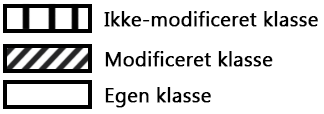
\includegraphics[scale=0.45]{Skraveringer}
\caption{Skraveringer i sekvensdiagrammer}
\label{Fig:Skraveringer}
\end{figure}


\subfile{LogiskView}

\newpage
\subfile{DeploymentView}

\newpage
\subfile{ProcessView}

\newpage
\subfile{ImplementationsView}

\newpage
\subfile{GenerelleDesignBeslutninger}



\end{document}